\documentclass[a4paper,12pt]{article}
\usepackage{graphicx}
\usepackage{amsmath}
\usepackage{geometry}
\usepackage{float}
\usepackage{tikz}

\providecommand{\brak}[1]{\ensuremath{\left(#1\right)}}
\geometry{margin=1in}

\title{Clock using Binary Logic in Arduino using AVR-GCC}
\author{EE24BTECH11001}
\date{\today}

\begin{document}

\maketitle

\section*{Overview}
\subsection*{Features}
The main features of the calculator are,
\begin{itemize}
    \item The entire code was written in AVR GCC.
    \item Instead of using $\mathbf{inc}$ command, k-maps were used. 
    \item The use of one decoder for each 7-segment display was avoided (only one decoder was used).

\end{itemize}
\subsection*{Hardware}

The hardware consists of:
\begin{table}[H]
\centering
\begin{tabular}{|c|l|}
\hline
\textbf{Quantity} & \textbf{Component} \\
\hline
6 & 7 Segment Display \\
\hline
1 & Arduino Uno\\
\hline
- & Wires \\
\hline
1 & Decoder (7447) \\
\hline
\end{tabular}
\caption{Materials Required}
\label{tab:materials}
\end{table}

\begin{itemize}
  \item Decrease requirement of multiple decoders, by intelligentally connecting the circuit as shown in the schematic and using \textbf{software multiplexing}
    Figure~\ref{fig:circuit_schematic}.
\end{itemize}
The schematic for connections is as shown below,
\begin{figure}[H]
    \centering
    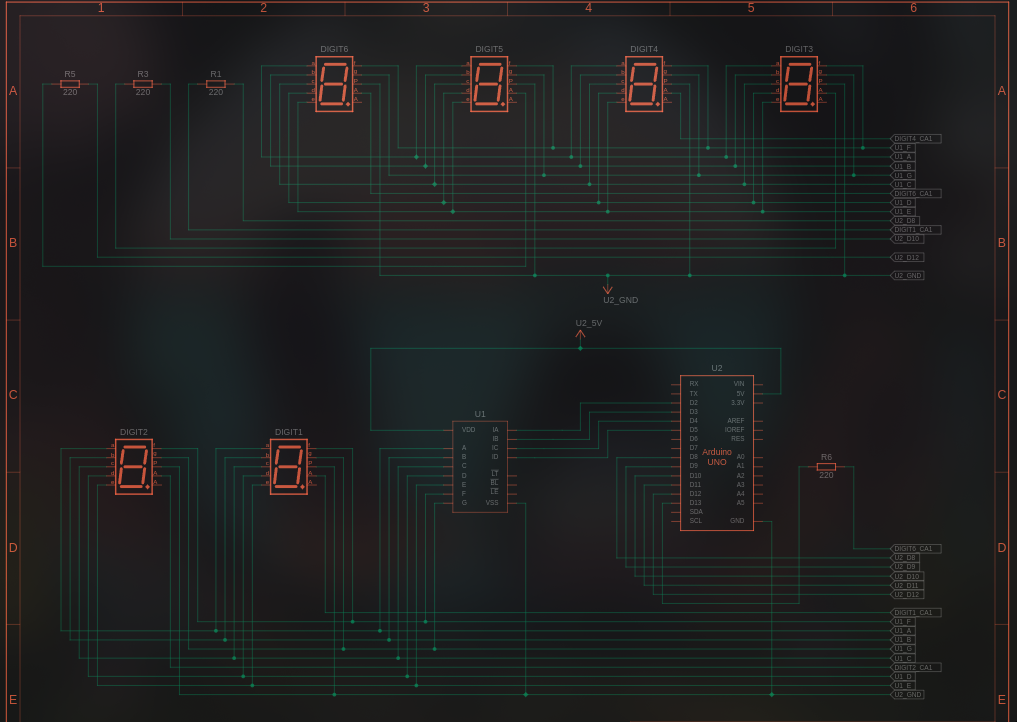
\includegraphics[width=\textwidth]{figs/circuit_schematic.png}
    \caption{Schematic of Circuit.}
    \label{fig:circuit_schematic}
\end{figure}
\begin{figure}
  \begin{center}
    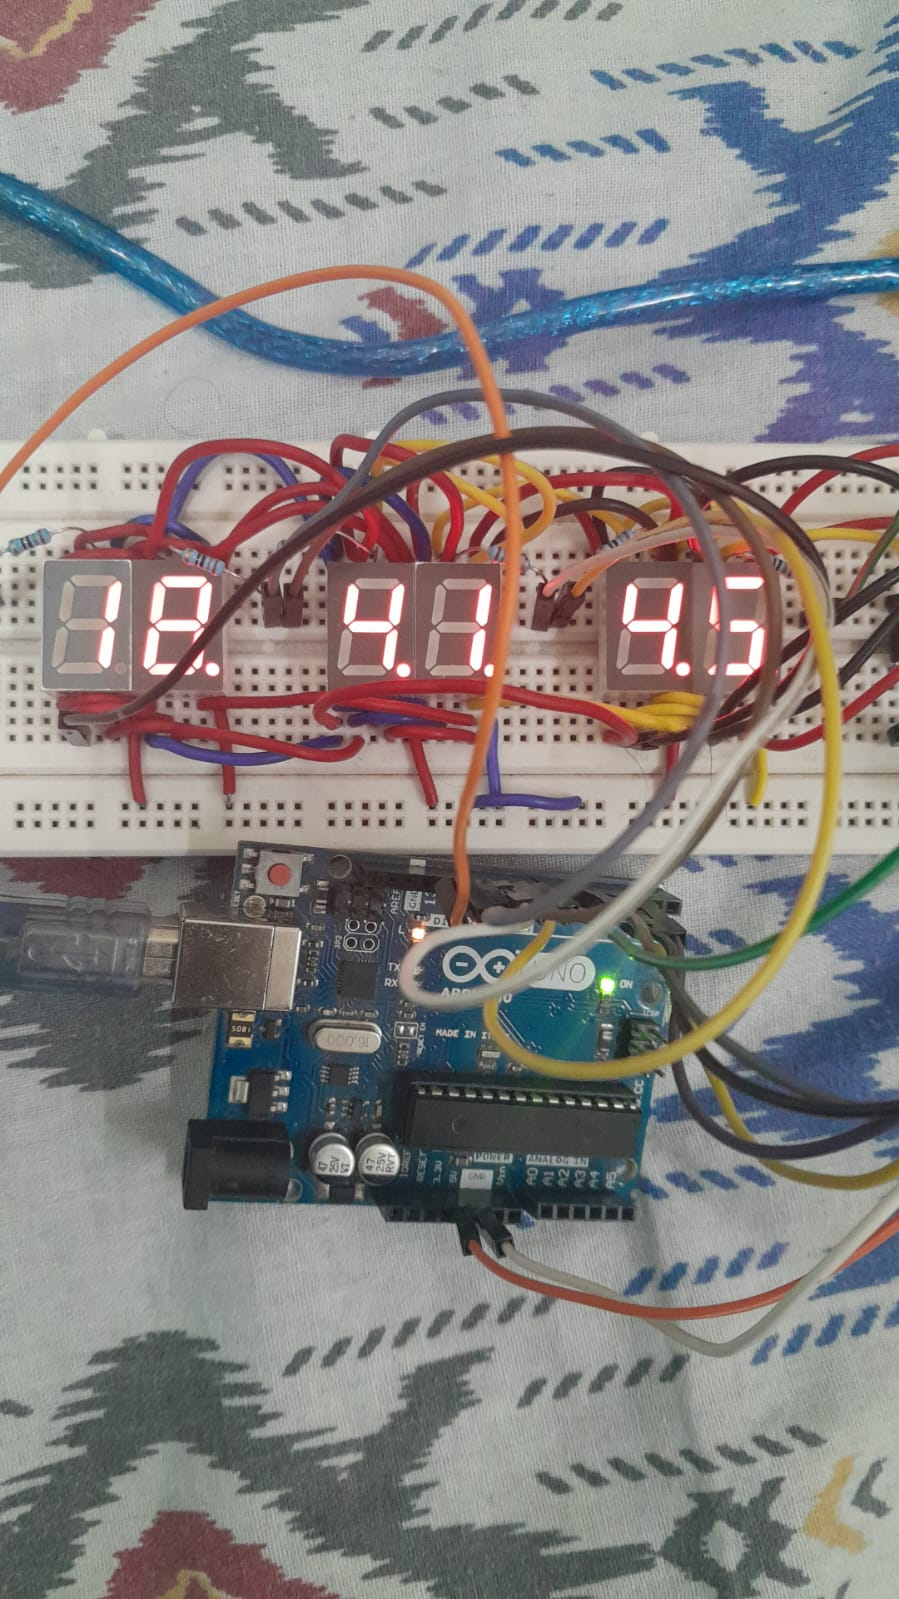
\includegraphics[width=0.95\textwidth]{figs/circuit_picture.jpeg}
  \end{center}
  \caption{}\label{fig:}
\end{figure}

\subsection*{Software Overview}
The software is implemented using AVR-GCC. The software trick used is called \textbf{software multiplexing}. The individual 7-segment-displays are connected to digital pins. The digital pins are cycled through at a very high rate $\left(\text{1 ms between two digitalWrite calls}\right)$, turning only 1 on at a time. At an appropriate delay of 1 second $\left(\text{realized using the Arduino's Counter}\right)$, all the values to be displayed are recalculated. This achieves the effect of a stationary
time which updates exactly at 1 second.
\section*{Timer}
Using multiple loops, a timer of one second was created. Within that one second, time is displayed (using the logic mentioned above), and at the end of one second, one's digit is incremented. The sub routine that does this has a piece of code at the end to increment ten's digit of seconds if incremented value of one's digit is 0. Similar the function to increment ten's digit has a line of code to increment one's digit of minutes if value after incrementing is 0. This is how time is incremented
\section*{Timer Initialization and Interrupt Handling}

The clock relies on precise timing through Timer1 and interrupt service routines:

\begin{verbatim}
    
void init_timer() {
    // Set CTC mode (Clear Timer on Compare Match)
    TCCR1B |= (1 << WGM12);
    
    // Set prescaler to 1024
    TCCR1B |= (1 << CS12) | (1 << CS10);

    // Set compare match value for 1s intervals (16MHz/1024)
    OCR1A = 15624;

    // Enable Timer1 compare match interrupt
    TIMSK1 |= (1 << OCIE1A);
    
    // Enable global interrupts
    sei();
}

// Interrupt Service Routine triggered every second
ISR(TIMER1_COMPA_vect) {
    flag = 1;  // Set flag to update clock values
}
\end{verbatim}

The timer operates in CTC mode with a 1024 prescaler, generating an interrupt every second. When the interrupt occurs, the ISR sets a flag that triggers the time update in the main loop, ensuring accurate timekeeping without blocking program execution.
\newline

This uses the Arduino's internal clock to achieve very minimal time losses.
\section*{Conclusion}
We achieved a fully functioning 24-hour clock using minimal number of BCD decoders by using software multiplexing in AVR-GCC using Arduino microcontroller.
\end{document}
